\documentclass[aspectratio=169, xcolor=dvipsnames]{beamer}

% --- Theme Setup ---
\usetheme{Madrid}
\usecolortheme{default}

% --- Packages ---
\usepackage{graphicx}
\usepackage{xcolor}
\usepackage{booktabs}
\usepackage{hyperref}
\usepackage{adjustbox}
\usepackage{amssymb}
\usepackage{longtable}
\usepackage{caption}

% --- Title Information ---
\title{Module 04}
\subtitle{Introduction to DBMS/1}
\author{Milav Dabgar}
\institute{www.milav.in}
\date{\today}

\begin{document}

% Title Slide
\begin{frame}
    \titlepage
\end{frame}

\begin{frame}{Module Recap}
    \begin{itemize}
        \item Comparison of data management using Python \& files and DBMS
        \item Efficacy and Efficient DBMS highlighted
    \end{itemize}
\end{frame}

\begin{frame}{Module Objectives}
    \begin{itemize}
        \item To familiarize with the basic notions and terminology of database management systems
        \item To understand the role of data models and languages
        \item To understand the approaches to database design
    \end{itemize}
\end{frame}

\begin{frame}{Module Outline}
    \begin{itemize}
        \item Levels of Abstraction
        \item Schema \& Instance
        \item Data Models
        \item Relational Databases
        \item DDL \& DML
        \item SQL
        \item Database Design
    \end{itemize}
\end{frame}

\section{Levels of Abstraction}

\begin{frame}
  \vfill
  \centering
  \begin{beamercolorbox}[sep=8pt,center,shadow=true,rounded=true]{title}
    \usebeamerfont{title}Levels of Abstraction\par%
  \end{beamercolorbox}
  \vfill
\end{frame}

\begin{frame}[fragile]{Levels of Abstraction}
    \begin{itemize}
        \item \textbf{Physical level:} describes how a record (for example, instructor) is stored
        \item \textbf{Logical level:} describes data stored in database, and the relationships among the data fields
    \end{itemize}
    
    \begin{verbatim}
type instructor = record
    ID        : string;
    name      : string;
    dept_name : string;
    salary    : integer;
end;
    \end{verbatim}
    
    \begin{itemize}
        \item \textbf{View level:} application programs hide details of data types
        \item Views can also hide information (such as an employee's salary) for security purposes
    \end{itemize}
\end{frame}

\begin{frame}{View of Data (An architecture for a database system)}
    \begin{center}
        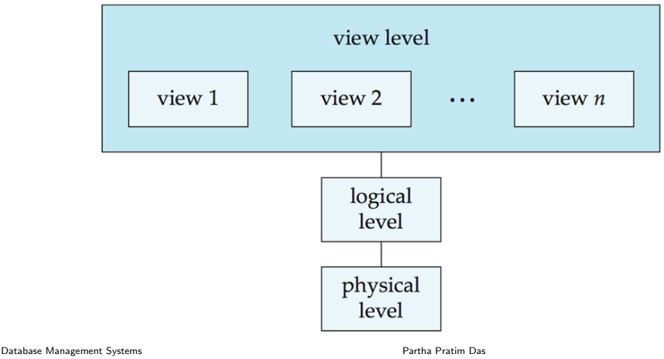
\includegraphics[height=0.7\textheight, width=0.9\textwidth, keepaspectratio]{../Lecture 1.4 - Intro to DBMS1_artifacts/image_000007_d5c77fd61bf3f2828a793ed48281b4a40ffd2712ba2db02bf234c2b1c8793d4a.png}
    \end{center}
\end{frame}

\section{Schema and Instance}

\begin{frame}
  \vfill
  \centering
  \begin{beamercolorbox}[sep=8pt,center,shadow=true,rounded=true]{title}
    \usebeamerfont{title}Schema and Instance\par%
  \end{beamercolorbox}
  \vfill
\end{frame}

\begin{frame}{Schemas and Instances}
    \begin{itemize}
        \item Similar to type of a variable and value of the variable at run-time in programming languages
        \item \textbf{Schema}
        \begin{itemize}
            \item \textbf{Logical Schema} -- the overall logical structure of the database
            \begin{itemize}
                \item[$\triangleright$] Analogous to type information of a variable in a program
                \item[$\triangleright$] \textbf{Example:} The database consists of information about a set of customers and accounts in a bank and the relationship between them
            \end{itemize}
            \item \textbf{Physical Schema} -- the overall physical structure of the database
        \end{itemize}
    \end{itemize}
    
    \vspace{1em}
    \begin{center}
        \begin{adjustbox}{max width=\textwidth}
        \begin{tabular}{|l|l|l|l|l|l|}
        \hline
        $\triangleright$ \textbf{Customer Schema} & Customer ID & Account \# & Aadhaar ID & Mobile \# & \\ \hline
        $\triangleright$ \textbf{Account Schema} & Account \# & Account Type & Interest Rate & Min. Bal. & Balance \\ \hline
        \end{tabular}
        \end{adjustbox}
    \end{center}
\end{frame}

\begin{frame}{Schemas and Instances (2)}
    \begin{itemize}
        \item \textbf{Instance}
        \begin{itemize}
            \item The actual content of the database at a particular point in time
            \item Analogous to the value of a variable
        \end{itemize}
    \end{itemize}
    
    \vspace{0.5em}
    \textbf{Customer Instance}
    \begin{center}
        \begin{adjustbox}{max width=\textwidth}
        \begin{tabular}{|l|l|l|l|l|}
        \hline
        \textbf{Name} & \textbf{Customer ID} & \textbf{Account \#} & \textbf{Aadhaar ID} & \textbf{Mobile \#} \\ \hline
        Pavan Laha & 6728 & 917322 & 182719289372 & 9830100291 \\ \hline
        Lata Kala & 8912 & 827183 & 918291204829 & 7189203928 \\ \hline
        Nand Prabhu & 6617 & 372912 & 127837291021 & 8892021892 \\ \hline
        \end{tabular}
        \end{adjustbox}
    \end{center}
    
    \vspace{0.5em}
    \textbf{Account Instance}
    \begin{center}
        \begin{adjustbox}{max width=\textwidth}
        \begin{tabular}{|l|l|l|l|l|}
        \hline
        \textbf{Account \#} & \textbf{Account Type} & \textbf{Interest Rate} & \textbf{Min. Bal.} & \textbf{Balance} \\ \hline
        917322 & Savings & 4.0\% & 5000 & 7812 \\ \hline
        372912 & Current & 0.0\% & & 291820 \\ \hline
        827183 & Term Deposit & & 10000 & 100000 \\ \hline
        \end{tabular}
        \end{adjustbox}
    \end{center}
\end{frame}

\begin{frame}{Schema and Instances}
    \begin{itemize}
        \item \textbf{Physical Data Independence} -- the ability to modify the physical schema without changing the logical schema
        \begin{itemize}
            \item Analogous to independence of Interface and Implementation in Object-Oriented Systems
            \item Applications depend on the logical schema
        \end{itemize}
        \item In general, the interfaces between the various levels and components should be well defined so that changes in some parts do not seriously influence others.
    \end{itemize}
\end{frame}

\section{Data Models}

\begin{frame}
  \vfill
  \centering
  \begin{beamercolorbox}[sep=8pt,center,shadow=true,rounded=true]{title}
    \usebeamerfont{title}Data Models\par%
  \end{beamercolorbox}
  \vfill
\end{frame}

\begin{frame}{Data Models}
    \begin{itemize}
        \item A collection of tools for describing
        \begin{itemize}
            \item Data
            \item Data relationships
            \item Data semantics
            \item Data constraints
        \end{itemize}
        \item Relational model (we focus in this course)
        \item Entity-Relationship data model (mainly for database design)
        \item Object-based data models (Object-oriented and Object-relational)
        \item Other older models
        \begin{itemize}
            \item Network model
            \item Hierarchical model
        \end{itemize}
        \item Recent models for Semi-structured or Unstructured data
        \begin{itemize}
            \item Converted to easily manageable formats
            \item Content Addressable Storage (CAS) with metadata descriptors
            \item XML format
            \item DBMS which supports BLOBs
        \end{itemize}
    \end{itemize}
\end{frame}

\begin{frame}{Data Models (2)}
    \begin{center}
        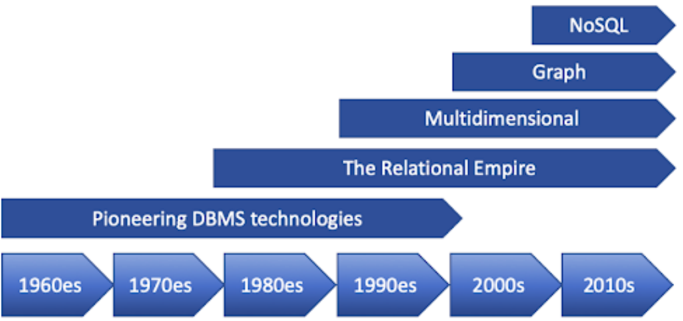
\includegraphics[height=0.7\textheight, width=0.9\textwidth, keepaspectratio]{../Lecture 1.4 - Intro to DBMS1_artifacts/image_000015_1c554f52c1dccb0ab2ffbac86b8fbb70fdc9fbc2ff7d1d5f0ef08bfda34396f7.png}
    \end{center}
\end{frame}

\begin{frame}{Relational Model}
    \begin{itemize}
        \item All the data is stored in various tables
        \item Example of tabular data in the relational model
    \end{itemize}
    
    \vspace{0.5em}
    \begin{center}
        \textbf{(a) The instructor table}
    \end{center}
    \begin{center}
        \begin{adjustbox}{max width=\textwidth}
        \begin{tabular}{|l|l|l|l|}
        \hline
        \textbf{ID} & \textbf{name} & \textbf{dept\_name} & \textbf{salary} \\ \hline
        22222 & Einstein & Physics & 95000 \\ \hline
        12121 & Wu & Finance & 90000 \\ \hline
        32343 & El Said & History & 60000 \\ \hline
        45565 & Katz & Comp. Sci. & 75000 \\ \hline
        98345 & Kim & Elec. Eng. & 80000 \\ \hline
        76766 & Crick & Biology & 72000 \\ \hline
        10101 & Srinivasan & Comp. Sci. & 65000 \\ \hline
        58583 & Califieri & History & 62000 \\ \hline
        83821 & Brandt & Comp. Sci. & 92000 \\ \hline
        15151 & Mozart & Music & 40000 \\ \hline
        33456 & Gold & Physics & 87000 \\ \hline
        76543 & Singh & Finance & 80000 \\ \hline
        \end{tabular}
        \end{adjustbox}
    \end{center}
\end{frame}

\begin{frame}{A Sample Relational Database}
    \begin{columns}
        \begin{column}{0.5\textwidth}
            \textbf{(a) The instructor table}
            \begin{center}
                \begin{adjustbox}{max width=\textwidth}
                \begin{tabular}{|l|l|l|l|}
                \hline
                \textbf{ID} & \textbf{name} & \textbf{dept\_name} & \textbf{salary} \\ \hline
                22222 & Einstein & Physics & 95000 \\ \hline
                12121 & Wu & Finance & 90000 \\ \hline
                32343 & El Said & History & 60000 \\ \hline
                \dots & \dots & \dots & \dots \\ \hline
                \end{tabular}
                \end{adjustbox}
            \end{center}
        \end{column}
        \begin{column}{0.5\textwidth}
            \textbf{(b) The department table}
            \begin{center}
                \begin{adjustbox}{max width=\textwidth}
                \begin{tabular}{|l|l|l|}
                \hline
                \textbf{dept\_name} & \textbf{building} & \textbf{budget} \\ \hline
                Comp. Sci. & Taylor & 100000 \\ \hline
                Biology & Watson & 90000 \\ \hline
                Elec. Eng. & Taylor & 85000 \\ \hline
                Music & Packard & 80000 \\ \hline
                Finance & Painter & 120000 \\ \hline
                History & Painter & 50000 \\ \hline
                Physics & Watson & 70000 \\ \hline
                \end{tabular}
                \end{adjustbox}
            \end{center}
        \end{column}
    \end{columns}
\end{frame}

\section{DDL and DML}

\begin{frame}
  \vfill
  \centering
  \begin{beamercolorbox}[sep=8pt,center,shadow=true,rounded=true]{title}
    \usebeamerfont{title}DDL and DML\par%
  \end{beamercolorbox}
  \vfill
\end{frame}

\begin{frame}[fragile]{Data Definition Language (DDL)}
    \begin{itemize}
        \item Specification notation for defining the database schema
        \item Example:
    \end{itemize}
    \begin{verbatim}
create table instructor ( 
    ID          char(5), 
    name        varchar(20), 
    dept_name   varchar(20), 
    salary      numeric(8,2)
)
    \end{verbatim}
    \begin{itemize}
        \item DDL compiler generates a set of table templates stored in a data dictionary
        \item Data dictionary contains metadata (that is, data about data)
        \begin{itemize}
            \item Database schema
            \item Integrity constraints
            \begin{itemize}
                \item[$\triangleright$] Primary key (ID uniquely identifies instructors)
            \end{itemize}
            \item Authorization
            \begin{itemize}
                \item[$\triangleright$] Who can access what
            \end{itemize}
        \end{itemize}
    \end{itemize}
\end{frame}

\begin{frame}{Data Manipulation Language (DML)}
    \begin{itemize}
        \item Language for accessing and manipulating the data organized by the appropriate data model
        \item DML: also known as Query Language
        \item Two classes of languages
        \begin{itemize}
            \item \textbf{Pure} -- used for proving properties about computational power and for optimization
            \begin{itemize}
                \item[$\triangleright$] \textbf{Relational Algebra (we focus in this course)}
                \item[$\triangleright$] Tuple relational calculus
                \item[$\triangleright$] Domain relational calculus
            \end{itemize}
            \item \textbf{Commercial} -- used in commercial systems
            \begin{itemize}
                \item[$\triangleright$] \textbf{SQL is the most widely used commercial language}
            \end{itemize}
        \end{itemize}
    \end{itemize}
\end{frame}

\section{SQL}

\begin{frame}
  \vfill
  \centering
  \begin{beamercolorbox}[sep=8pt,center,shadow=true,rounded=true]{title}
    \usebeamerfont{title}SQL\par%
  \end{beamercolorbox}
  \vfill
\end{frame}

\begin{frame}{SQL}
    \begin{itemize}
        \item The most widely used commercial language
        \item SQL is \textbf{NOT} a Turing Machine equivalent language
        \begin{itemize}
            \item Cannot be used to solve all problems that a C program, for example, can solve
            \item To be able to compute complex functions, SQL is usually embedded in some higher-level language
        \end{itemize}
        \item Application programs generally access databases through one of:
        \begin{itemize}
            \item Language extensions to allow embedded SQL
            \item Application Programming Interface or API (for example, ODBC/JDBC) which allow SQL queries to be sent to a database
        \end{itemize}
    \end{itemize}
\end{frame}

\section{Database Design}

\begin{frame}
  \vfill
  \centering
  \begin{beamercolorbox}[sep=8pt,center,shadow=true,rounded=true]{title}
    \usebeamerfont{title}Database Design\par%
  \end{beamercolorbox}
  \vfill
\end{frame}

\begin{frame}{Database Design}
    The process of designing the general structure of the database:
    \begin{itemize}
        \item \textbf{Logical Design} -- Deciding on the database schema. Database design requires that we find a good collection of relation schema
        \begin{itemize}
            \item Business decision
            \begin{itemize}
                \item[$\triangleright$] What attributes should we record in the database?
            \end{itemize}
            \item Computer Science decision
            \begin{itemize}
                \item[$\triangleright$] What relation schemas should we have and how should the attributes be distributed among the various relation schemas?
            \end{itemize}
        \end{itemize}
        \item \textbf{Physical Design} -- Deciding on the physical layout of the database
    \end{itemize}
\end{frame}

\begin{frame}{Database Design (2)}
    \textbf{Is there any problem with this relation?}
    \vspace{0.5em}
    \begin{center}
        \begin{adjustbox}{max width=\textwidth}
        \begin{tabular}{|l|l|l|l|l|l|}
        \hline
        \textbf{ID} & \textbf{name} & \textbf{salary} & \textbf{dept\_name} & \textbf{building} & \textbf{budget} \\ \hline
        22222 & Einstein & 95000 & Physics & Watson & 70000 \\ \hline
        12121 & Wu & 90000 & Finance & Painter & 120000 \\ \hline
        32343 & El Said & 60000 & History & Painter & 50000 \\ \hline
        45565 & Katz & 75000 & Comp. Sci. & Taylor & 100000 \\ \hline
        98345 & Kim & 80000 & Elec. Eng. & Taylor & 85000 \\ \hline
        76766 & Crick & 72000 & Biology & Watson & 90000 \\ \hline
        10101 & Srinivasan & 65000 & Comp. Sci. & Taylor & 100000 \\ \hline
        58583 & Califieri & 62000 & History & Painter & 50000 \\ \hline
        83821 & Brandt & 92000 & Comp. Sci. & Taylor & 100000 \\ \hline
        15151 & Mozart & 40000 & Music & Packard & 80000 \\ \hline
        33456 & Gold & 87000 & Physics & Watson & 70000 \\ \hline
        76543 & Singh & 80000 & Finance & Painter & 120000 \\ \hline
        \end{tabular}
        \end{adjustbox}
    \end{center}
\end{frame}

\begin{frame}{Module Summary}
    \begin{itemize}
        \item Familiarized with the basic notions and terminology of database management systems
        \item Introduced the role of data models and languages
        \item Introduced the approaches to database design
    \end{itemize}
    
    \vspace{2em}
    \begin{center}
    \small \textit{Slides used in this presentation are borrowed from \url{http://db-book.com/} with kind permission of the authors.} \\
    \small \textit{Edited and new slides are marked with 'PPD'.}
    \end{center}
\end{frame}

\end{document}
